%Este trabalho está licenciado sob a Licença Atribuição-CompartilhaIgual 4.0 Internacional Creative Commons. Para visualizar uma cópia desta licença, visite http://creativecommons.org/licenses/by-sa/4.0/deed.pt_BR ou mande uma carta para Creative Commons, PO Box 1866, Mountain View, CA 94042, USA.

\chapter{Estudo de planos}\label{cap_ep}
\thispagestyle{fancy}

\ifispython
\begin{obs}\label{obs:cap_ep_py}
  Neste capítulo, assumimos que os códigos \verb+Python+ têm o seguinte preambulo:
\begin{verbatim}
from sympy import *
from sympy.plotting import plot3d_parametric_line
\end{verbatim}
\end{obs}
\fi

\section{Equações do plano}\label{cap_ep_sec_eqsplano}

Um plano $\pi$ fica unicamente determinado por um ponto $A\in \pi$ e dois vetores linearmente independentes $\vec{u},\vec{v}\in \pi$\footnote{No sentido que $\vec{u}$ e $\vec{v}$ têm representantes no plano $\pi$.}.

\subsection{Equação vetorial do plano}

Consideremos um plano $\pi$ determinado pelo ponto $A$ e os vetores $\vec{u}$ e $\vec{v}$. Então, um ponto $P\in \pi$ se, e somente se, $\overrightarrow{AP}$ é coplanar a $\vec{u}$ e $\vec{v}$, i.e. $\overrightarrow{AP}$, $\vec{u}$ e $\vec{v}$ são linearmente dependentes. Ou seja,
\begin{equation}
  P\in\pi \Leftrightarrow \overrightarrow{AP} = \lambda\vec{u}+\beta\vec{v},\quad\lambda,\beta\in\mathbb{R},
\end{equation}
esta última é chamada de \emph{equação vetorial do plano}.

\begin{ex}\label{ex:ep_vet}
  Consideremos o plano $\pi$ determinado pelo ponto $A = (1,-1,1)$ e pelos vetores $\vec{u} = (2,-1,0)$ e $\vec{v} = (0,1,1)$ (Veja a Figura \ref{fig:ex_ep_vet}. Desta forma, uma equação vetorial para este plano é
  \begin{equation}
    \overrightarrow{AP} = \lambda\vec{u}+\beta\vec{v},
  \end{equation}
  para $\lambda,\beta\in\mathbb{R}$.
  
  \begin{figure}[H]
    \centering
    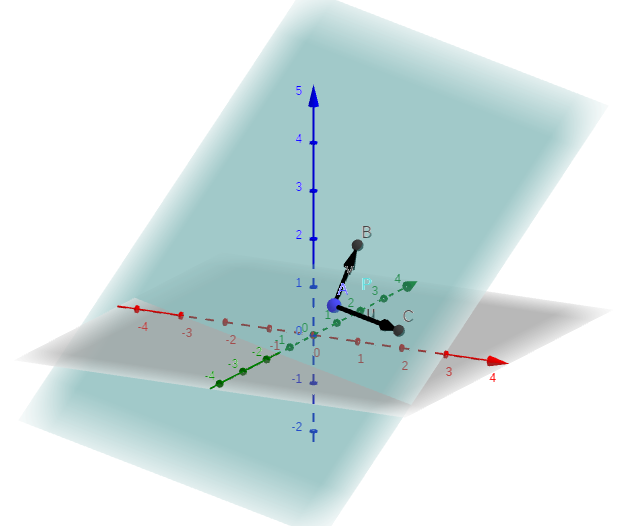
\includegraphics[width=0.7\textwidth]{./cap_ep/dados/fig_ex_ep_vet/fig_ex_ep_vet}
    \caption{Esboço do plano $\pi$ discutido no Exemplo \ref{ex:ep_vet}.}
    \label{fig:ex_ep_vet}
  \end{figure}
  
  Tomando, por exemplo, $\lambda = -1$ e $\beta = 1$, obtemos
  \begin{align}
    \overrightarrow{AP} &= \lambda\vec{u}+\beta\vec{v}\\
                        &= -(2,-1,0) + (0,1,1)\\
                        &= (-2,2,1).
  \end{align}
  Observando que as coordenadas do ponto $P$ são iguais as coordenadas do vetor $\overrightarrow{OP}$, temos
  \begin{align}
    \overrightarrow{OP} &= \overrightarrow{OA}+\overrightarrow{AP}\\
                        &= (1,-1,1)+(-2,2,1)\\
                        &= (-1,1,2).
  \end{align}
  Ou seja, $P = (-1,1,2)\in\pi$.
\end{ex}

\subsection{Equações paramétricas do plano}

Seja um plano $\pi$ com $A=(x_A,y_A,z_A)\in\pi$ e os vetores $\vec{u}=(u_1,u_2,u_3)\in\pi$ e $\vec{v}=(v_1,v_2,v_3)\in\pi$ linearmente independentes. Então, todo o ponto $P=(x,y,z)$ do plano $\pi$ satisfaz
\begin{equation}
  \overrightarrow{AP} = \lambda\vec{u}+\beta\vec{v},
\end{equation}
para dados parâmetros $\lambda,\beta\in\mathbb{R}$. Assim, temos
\begin{align}
  (x-x_A,y-y_A,z-z_A) &= \lambda(u_1,u_2,u_3)+\beta(v_1,v_2,v_3)\\
                      &= (\lambda u_1+\beta v_1,\lambda u_2+\beta v_2,\lambda u_3+\beta v_3).
\end{align}
Portanto, temos
\begin{align}
  x-x_A &= \lambda u_1+\beta v_1,\\
  y-y_A &= \lambda u_2+\beta v_2,\\
  z-z_A &= \lambda u_3+\beta v_3.
\end{align}
Ou, equivalentemente,
\begin{align}
  x &= x_A + \lambda u_1+\beta v_1,\\
  y &= y_A + \lambda u_2+\beta v_2,\\
  z &= z_A + \lambda u_3+\beta v_3,
\end{align}
as quais são chamadas de \emph{equações paramétricas do plano}.

\begin{ex}
  No Exemplo \ref{ex:ep_vet}, discutimos sobre o plano $\pi$ determinado pelo ponto $A = (1,-1,1)$ e os vetores $\vec{u}=(2,-1,0)$ e $\vec{v}=(0,1,1)$. Do que vimos acima, temos que
  \begin{align}
    x &= 1 + 2\lambda,\\
    y &= -1 -\lambda + \beta,\\
    z &= 1+\beta,
  \end{align}
  são equações paramétricas deste plano.

  \ifispython
  Podemos usar as equações paramétricas do plano para plotá-lo usando o \verb+Sympy+. Para tanto, podemos usar os seguintes comandos:
\begin{verbatim}
from sympy import *
from sympy.plotting import plot3d_parametric_surface
var('r,s',real=True)
plot3d_parametric_surface(1+2*r,-1-r+s,1+s,
                          (r,-2,2),(s,-2,2),show=True,
                          xlabel='$x$',ylabel='$y$')
\end{verbatim}
  \fi
\end{ex}

\subsection{Equação geral do plano}

Seja $\pi$ o plano determinado pelo ponto $A=(x_A,y_A,z_A)$ e pelos vetores $\vec{u}=(u_1,u_2,u_3)$ e $\vec{v} = (v_1,v_2,v_3)$. Sabemos que $P=(x,y,z)\in\pi$ se, e somente se, $\overrightarrow{AP}$, $\vec{u}$ e $\vec{v}$ são linearmente dependentes. Ou, equivalentemente, o produto misto $[\overrightarrow{AP},\vec{u},\vec{v}] = 0$. Logo,
\begin{align}
  0 &= [\overrightarrow{AP},\vec{u},\vec{v}] \\
    &=
      \begin{vmatrix}
        x-x_A & y-y_A & z-z_A \\
        u_1 & u_2 & u_3 \\
        v_1 & v_2 & v_3
      \end{vmatrix} \\
    &= -u_1v_2z_A + u_1v_3y_A + u_2v_1z_A \\
    &- u_2v_3x_A - u_3v_1y_A + u_3v_2x_A \\
    &+ x(u_2v_3 - u_3v_2) + y(-u_1v_3 + u_3v_1) + z(u_1v_2 - u_2v_1).
\end{align}
Observamos que a equação acima tem a forma geral
\begin{equation}
  ax + by + cz + d = 0,
\end{equation}
com $a,b,c,d$ não todos nulos ou, equivalentemente, $a^2+b^2+c^2+d^2\neq 0$. Esta última é chamada \emph{equação geral do plano}.

\begin{ex}
  No Exemplo \ref{ex:ep_vet}, discutimos sobre o plano $\pi$ determinado pelo ponto $A = (1,-1,1)$ e os vetores $\vec{u}=(2,-1,0)$ e $\vec{v}=(0,1,1)$. Para encontrarmos a equação geral deste plano, tomamos $P = (x,y,z)$ e calculamos
  \begin{align}
    0 &= [\overrightarrow{AP},\vec{u},\vec{v}]\\
      &=
        \begin{vmatrix}
          x-1 & y+1 & z-1 \\
          2 & -1 & 0 \\
          0 & 1 & 1
        \end{vmatrix}\\
      &= - x - 2 y + 2 z - 3.
  \end{align}
  Ou seja, a equação geral deste plano é
  \begin{equation}
    -x - 2y + 2z -3 = 0.
  \end{equation}
\end{ex}

\subsection{Exercícios resolvidos}

\begin{exeresol}
  Seja $\pi$ um plano tal que $A=(2,0,-1)\in\pi$, $P=(0,1,-1)\in\pi$ e $\vec{u}=(1,0,1)\in\pi$. Determine uma equação vetorial para $\pi$.
\end{exeresol}
\begin{resol}
  Para obtermos uma equação vetorial do plano $\pi$, precisamos de um ponto e dois vetores l.i. em $\pi$. Do enunciado, temos o ponto $A=(2,0,-1)\in\pi$ e o vetor $\vec{u}$. Portanto, precisamos encontrar um vetor $\vec{v}\in\pi$ tal que $\vec{u}$ e $\vec{v}$ sejam l.i.. Por sorte, temos $P=(0,1,-1)\in\pi$ e, portanto $\overrightarrow{AP}\in\pi$. Podemos tomar
  \begin{align}
    \vec{v} &= \overrightarrow{AP}\\
            &= (-2,1,0),
  \end{align}
  pois $\vec{v}$ e $\vec{u}$ são l.i.. Logo, uma equação vetorial do plano $pi$ é
  \begin{align}
    \overrightarrow{AP} &= \lambda\vec{u}+\beta\vec{v},\\
                        &= \lambda (1,0,1) + \beta (-2,1,0),
  \end{align}
  com $\lambda,\beta\in\mathbb{R}$.
\end{resol}

\begin{exeresol}
  Seja $\pi$ o plano de equações paramétricas
  \begin{align}
    x = -1 + \lambda,\\
    y = \beta,\\
    z = 1 - \lambda + \beta.
  \end{align}
  Determine o valor de $z_P$ de forma que $P=(-1,2,z_P)\in\pi$.
\end{exeresol}
\begin{resol}
  Para que $P=(-1,2,z_P)$ pertença ao plano, devemos ter
  \begin{align}
    -1 = -1 + \lambda,\\
    2 = \beta,\\
    z_P = 1 - \lambda + \beta.
  \end{align}
  Das duas primeiras equações, obtemos $\lambda=0$ e $\beta=2$. Daí, da terceira equação, temos
  \begin{align}
    z_P = 1 - 0 + 2 = 3.
  \end{align}
\end{resol}

\emconstrucao
